\subsection{数字滤波器的设计}

数字滤波器的设计分为两种,一种是\bd{有限脉冲响应}(FIR)滤波器的设计,
另一种是\bd{无限脉冲响应}(IIR)滤波器的设计。

\subsubsection{低通 FIR 滤波器的设计}

由于单位冲激响应被截短成了有限项,所以滤波器的频率响应特性会发生改变。
根据经验,在设计滤波器时, 理想低通滤波器的截止频率不使用通带边缘频率,
而是使用\bd{过渡带中点的频率}。即如图 \ref{fig:low_pass_filter_fir} 所示,
\begin{align*}
    f_c = \text{设计指标要求的通道边缘频率} + \frac{\text{过渡带宽度}}{2},
\end{align*}
其中 $f_c$ 是理想低通滤波器的截止频率。

\begin{figure}[H]
    \centering
    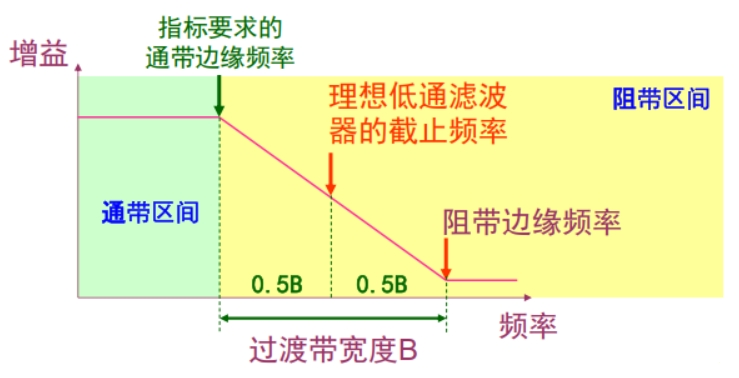
\includegraphics[width=0.8\textwidth]{chap4/img/low_pass_filter_fir.png}
    \caption{低通 FIR 滤波器设计}
    \label{fig:low_pass_filter_fir}
\end{figure}

\begin{example}[设计低通 FIR 滤波器的步骤]
    设计低通 FIR 滤波器的步骤如下:
    \begin{enumerate}
        \item 在过渡带宽度中间,选择理想低通滤波器的截止频率
            \begin{align*}
                f_c = \text{设计指标要求的通道边缘频率} + \frac{\text{过渡带宽度}}{2}.
            \end{align*}
        \item 计算截止频率的数字角频率
            \begin{align*}
                \omega_c = 2\pi \times \frac{f_c}{f_s},
            \end{align*}
            并代入
            \begin{align*}
                h(n) = \frac{\sin(\omega_c n)}{\pi n}.
            \end{align*}
        \item 从表中选择满足阻带衰减及其他要求的窗函数,计算窗内非零项的数目 $N$,
            选取满足条件的奇数 $N$,并计算窗函数 $w(n)$。
        \item 将 $w(n)$ 和 $h(n)$ 相乘,计算有限长脉冲响应 $h'(n) = w(n)h(n)$。
        \item 将脉冲右移 $(N - 1) / 2$ 个单位,得到 $h''(n)$。
    \end{enumerate}
\end{example}

\begin{example}
    根据下列指标设计低通 FIR 滤波器,写出其单位冲激响应函数 $h(n)$。
    \begin{figure}[H]
        \centering
        \begin{tabular}{|c|c|}
            \hline
            通带边缘频率:$10\;\mathrm{kHz}$ & 阻带边缘频率:$22\;\mathrm{kHz}$ \\
            \hline
            采样频率:$50\;\mathrm{kHz}$ & 阻带衰减:$75\;\mathrm{dB}$ \\
            \hline
        \end{tabular}
    \end{figure}
    供设计 FIR 滤波器时参考的各种窗函数性能如下图所示(若多种同时满足,则选序号最小的):
    \begin{figure}[H]
        \centering
        \begin{tabular}{|c|c|>{\centering\arraybackslash}p{5cm}|>{\centering\arraybackslash}p{4cm}|c|c|}
            \hline
            \textbf{序号} & \textbf{窗类型} & \makecell{\textbf{窗函数} \\ $(\abs{n} \le (N - 1) / 2)$} & \makecell{\textbf{窗内项数}\\(\text{T.W.} 是过渡带宽度)} & \textbf{阻带衰减} & \textbf{通带边缘增益} \\
            \hline
            1 & 矩形 & $1$ & $0.91 f_s / \text{T.W.}$ & $21$ & $-0.9$ \\
            \hline
            2 & 汉宁 & $0.5 + 0.5\cos(2\pi n / (N-1))$ & $3.32 f_s / \text{T.W.}$ & $44$ & $-0.06$ \\
            \hline
            3 & 哈明 & $0.54 + 0.46\cos(2\pi n / (N-1))$ & $3.44 f_s / \text{T.W.}$ & $55$ & $-0.02$ \\
            \hline
            4 & 布莱克曼 & $0.42 + 0.5\cos(2\pi n / (N-1)) + 0.08\cos(4\pi n / (N-1))$ & $5.98 f_s / \text{T.W.}$ & $75$ & $-0.0014$ \\
            \hline
        \end{tabular}
    \end{figure}
\end{example}

\begin{solution}
    过渡带宽度
    \begin{align*}
        \text{T.W.} = 22 - 10 = 12\;\mathrm{kHz},
    \end{align*}
    理想低通滤波器的截止频率
    \begin{align*}
        f_c = 10 + \frac{1}{2} \times 12 = 16\;\mathrm{kHz},
    \end{align*}
    则相应的数字角频率
    \begin{align*}
        \omega_c = 2\pi \times \frac{f_c}{f_s} = 2\pi \times \frac{16}{50} = \frac{16\pi}{25}.
    \end{align*}
    计算得
    \begin{align*}
        h(n) = \frac{\sin(\omega_c n)}{\pi n} = \frac{\sin(16\pi n / 25)}{\pi n}.
    \end{align*}
    由阻带衰减为 $75\;\mathrm{dB}$ 知,应当选择布莱克曼窗。由于
    \begin{align*}
        N \ge 5.98 \times \frac{f_s}{\text{T.W.}} = 5.98 \times \frac{50}{12} \approx 24.9,
    \end{align*}
    故取 $N = 25$。则
    \begin{align*}
        w(n) = 0.42 + 0.5\cos\frac{2\pi n}{N - 1} + 0.08\cos\frac{4\pi n}{N - 1} = 0.42 + 0.5\cos\frac{\pi n}{12} + 0.08\cos\frac{\pi n}{6}.
    \end{align*}
    因此,低通 FIR 滤波器的冲激响应函数为
    \begin{align*}
        h'(n) = h(n) w(n) = \frac{\sin(16\pi n / 25)}{\pi n} \left(0.42 + 0.5\cos\frac{\pi n}{12} + 0.08\cos\frac{\pi n}{6}\right) \quad (\abs{n} \le 12).
    \end{align*}
    将其右移 $(N - 1) / 2 = 12$ 个单位,即得
    \begin{align*}
        h''(n) = \frac{\sin(16\pi (n - 12) / 25)}{\pi (n - 12)} \left(0.42 + 0.5\cos\frac{\pi (n - 12)}{12} + 0.08\cos\frac{\pi (n - 12)}{6}\right) \quad (0 \le n \le 24).
    \end{align*}
\end{solution}

\begin{exercise}
    根据下列指标设计低通 FIR 滤波器,写出其单位冲激响应函数 $h(n)$。
    \begin{figure}[H]
        \centering
        \begin{tabular}{|c|c|}
            \hline
            通带边缘频率:$2\;\mathrm{kHz}$ & 阻带边缘频率:$3\;\mathrm{kHz}$ \\
            \hline
            采样频率:$10\;\mathrm{kHz}$ & 阻带衰减:$40\;\mathrm{dB}$ \\
            \hline
        \end{tabular}
    \end{figure}
    供设计 FIR 滤波器时参考的各种窗函数性能如下图所示(若多种同时满足,则选序号最小的):
    \begin{figure}[H]
        \centering
        \begin{tabular}{|c|c|>{\centering\arraybackslash}p{5cm}|>{\centering\arraybackslash}p{4cm}|c|c|}
            \hline
            \textbf{序号} & \textbf{窗类型} & \makecell{\textbf{窗函数} \\ $(\abs{n} \le (N - 1) / 2)$} & \makecell{\textbf{窗内项数}\\(\text{T.W.} 是过渡带宽度)} & \textbf{阻带衰减} & \textbf{通带边缘增益} \\
            \hline
            1 & 矩形 & $1$ & $0.91 f_s / \text{T.W.}$ & $21$ & $-0.9$ \\
            \hline
            2 & 汉宁 & $0.5 + 0.5\cos(2\pi n / (N-1))$ & $3.32 f_s / \text{T.W.}$ & $44$ & $-0.06$ \\
            \hline
            3 & 哈明 & $0.54 + 0.46\cos(2\pi n / (N-1))$ & $3.44 f_s / \text{T.W.}$ & $55$ & $-0.02$ \\
            \hline
            4 & 布莱克曼 & $0.42 + 0.5\cos(2\pi n / (N-1)) + 0.08\cos(4\pi n / (N-1))$ & $5.98 f_s / \text{T.W.}$ & $75$ & $-0.0014$ \\
            \hline
        \end{tabular}
    \end{figure}
\end{exercise}

\begin{solution}
    过渡带宽度
    \begin{align*}
        \text{T.W.} = 3 - 2 = 1\;\mathrm{kHz},
    \end{align*}
    理想低通滤波器的截止频率
    \begin{align*}
        f_c = 2 + \frac{1}{2} \times 2 = 2.5\;\mathrm{kHz},
    \end{align*}
    则相应的数字角频率
    \begin{align*}
        \omega_c = 2\pi \times \frac{f_c}{f_s} = 2\pi \times \frac{2.5}{10} = \frac{\pi}{2}.
    \end{align*}
    计算得
    \begin{align*}
        h(n) = \frac{\sin(\omega_c n)}{\pi n} = \frac{\sin(\pi n / 2)}{\pi n}.
    \end{align*}
    由阻带衰减为 $40\;\mathrm{dB}$ 知,应当选择汉宁窗。由于
    \begin{align*}
        N \ge 3.32 \times \frac{f_s}{\text{T.W.}} = 3.32 \times \frac{10}{1} = 33.2,
    \end{align*}
    故取 $N = 35$。则
    \begin{align*}
        w(n) = 0.5 + 0.5\cos\frac{2\pi n}{N - 1} = 0.5 + 0.5\cos\frac{\pi n}{17}.
    \end{align*}
    因此,低通 FIR 滤波器的冲激响应函数为
    \begin{align*}
        h'(n) = h(n) w(n) = \frac{\sin(\pi n / 2)}{\pi n} \left(0.5 + 0.5\cos\frac{\pi n}{17}\right) \quad (\abs{n} \le 17).
    \end{align*}
    将其右移 $(N - 1) / 2 = 17$ 个单位,即得
    \begin{align*}
        h''(n) = \frac{\sin(\pi (n - 17) / 2)}{\pi (n - 17)} \left(0.5 + 0.5\cos\frac{\pi (n - 17)}{17}\right) \quad (0 \le n \le 34).
    \end{align*}
\end{solution}

\begin{exercise}
    根据下列指标设计低通 FIR 滤波器,写出其单位冲激响应函数 $h(n)$。
    \begin{figure}[H]
        \centering
        \begin{tabular}{|c|c|}
            \hline
            通带边缘频率:$3.3\;\mathrm{kHz}$ & 过渡带宽度:$4.4\;\mathrm{kHz}$ \\
            \hline
            采样频率:$22\;\mathrm{kHz}$ & 阻带衰减:$43\;\mathrm{dB}$ \\
            \hline
        \end{tabular}
    \end{figure}
    供设计 FIR 滤波器时参考的各种窗函数性能如下图所示(若多种同时满足,则选序号最小的):
    \begin{figure}[H]
        \centering
        \begin{tabular}{|c|c|>{\centering\arraybackslash}p{5cm}|>{\centering\arraybackslash}p{4cm}|c|c|}
            \hline
            \textbf{序号} & \textbf{窗类型} & \makecell{\textbf{窗函数} \\ $(\abs{n} \le (N - 1) / 2)$} & \makecell{\textbf{窗内项数}\\(\text{T.W.} 是过渡带宽度)} & \textbf{阻带衰减} & \textbf{通带边缘增益} \\
            \hline
            1 & 矩形 & $1$ & $0.91 f_s / \text{T.W.}$ & $21$ & $-0.9$ \\
            \hline
            2 & 汉宁 & $0.5 + 0.5\cos(2\pi n / (N-1))$ & $3.32 f_s / \text{T.W.}$ & $44$ & $-0.06$ \\
            \hline
            3 & 哈明 & $0.54 + 0.46\cos(2\pi n / (N-1))$ & $3.44 f_s / \text{T.W.}$ & $55$ & $-0.02$ \\
            \hline
            4 & 布莱克曼 & $0.42 + 0.5\cos(2\pi n / (N-1)) + 0.08\cos(4\pi n / (N-1))$ & $5.98 f_s / \text{T.W.}$ & $75$ & $-0.0014$ \\
            \hline
        \end{tabular}
    \end{figure}
\end{exercise}

\begin{solution}
    截止频率
    \begin{align*}
        f_c = 3.3 + \frac{1}{2} \times 4.4 = 5.5\;\mathrm{kHz},
    \end{align*}
    则
    \begin{align*}
        \omega_c = 2\pi \times \frac{f_c}{f_s} = 2\pi \times \frac{5.5}{22} = \frac{\pi}{2}.
    \end{align*}
    计算得
    \begin{align*}
        h(n) = \frac{\sin(\omega_c n)}{\pi n} = \frac{\sin(\pi n / 2)}{\pi n}.
    \end{align*}
    由阻带衰减为 $43\;\mathrm{dB}$ 知,应当选择汉宁窗。由于
    \begin{align*}
        N \ge 3.32 \times \frac{f_s}{\text{T.W.}} = 3.32 \times \frac{22}{4.4} = 16.6,
    \end{align*}
    故取 $N = 17$。则
    \begin{align*}
        w(n) = 0.5 + 0.5\cos\frac{2\pi n}{N - 1} = 0.5 + 0.5\cos\frac{\pi n}{8}.
    \end{align*}
    因此,低通 FIR 滤波器的冲激响应函数为
    \begin{align*}
        h'(n) = h(n) w(n) = \frac{\sin(\pi n / 2)}{\pi n} \left(0.5 + 0.5\cos\frac{\pi n}{8}\right) \quad (\abs{n} \le 8).
    \end{align*}
    将其右移 $(N - 1) / 2 = 8$ 个单位,即得
    \begin{align*}
        h''(n) = \frac{\sin(\pi (n - 8) / 2)}{\pi (n - 8)} \left(0.5 + 0.5\cos\frac{\pi (n - 8)}{8}\right) \quad (0 \le n \le 16).
    \end{align*}
\end{solution}

\subsubsection{带通 FIR 滤波器的设计}

频率响应函数需要在频域移动到新的位置,频移的方法:将脉冲响应与余弦函数相乘:
\begin{align*}
    h'(n) = h(n)w(n)\cos(\omega_0 n),
\end{align*}
其中 $w(n)$ 是窗函数,$\omega_0$ 是带通滤波器的中心频率,如图 \ref{fig:band-pass-filter-fir} 所示。

\begin{figure}[H]
    \centering
    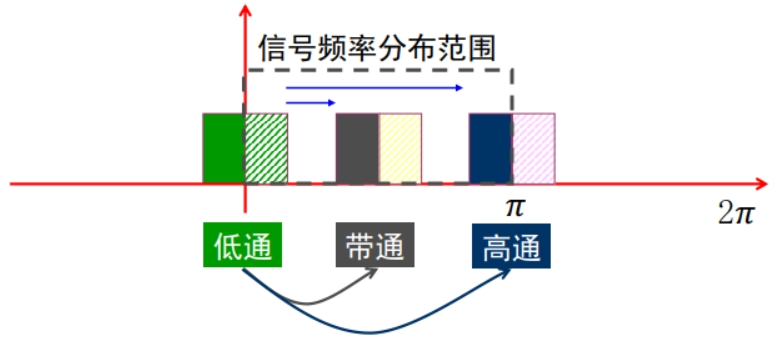
\includegraphics[width=0.8\textwidth]{chap4/img/band_pass_filter_fir.png}
    \caption{带通 FIR 滤波器设计}
    \label{fig:band-pass-filter-fir}
\end{figure}

\begin{exercise}
    根据下列指标设计带通 FIR 滤波器,写出其单位冲激响应函数 $h(n)$。
    \begin{figure}[H]
        \centering
        \begin{tabular}{|c|c|}
            \hline
            带通中心频率:$4\;\mathrm{kHz}$ & 过渡带宽度:$0.5\;\mathrm{kHz}$ \\
            \hline
            通带边缘频率:$3.5\;\mathrm{kHz}, 4.5\;\mathrm{kHz}$ & 阻带衰减:$50\;\mathrm{dB}$ \\
            \hline
            采样频率:$22\;\mathrm{kHz}$ & \\
            \hline
        \end{tabular}
    \end{figure}
    供设计 FIR 滤波器时参考的各种窗函数性能如下图所示(若多种同时满足,则选序号最小的):
    \begin{figure}[H]
        \centering
        \begin{tabular}{|c|c|>{\centering\arraybackslash}p{5cm}|>{\centering\arraybackslash}p{4cm}|c|c|}
            \hline
            \textbf{序号} & \textbf{窗类型} & \makecell{\textbf{窗函数} \\ $(\abs{n} \le (N - 1) / 2)$} & \makecell{\textbf{窗内项数}\\(\text{T.W.} 是过渡带宽度)} & \textbf{阻带衰减} & \textbf{通带边缘增益} \\
            \hline
            1 & 矩形 & $1$ & $0.91 f_s / \text{T.W.}$ & $21$ & $-0.9$ \\
            \hline
            2 & 汉宁 & $0.5 + 0.5\cos(2\pi n / (N-1))$ & $3.32 f_s / \text{T.W.}$ & $44$ & $-0.06$ \\
            \hline
            3 & 哈明 & $0.54 + 0.46\cos(2\pi n / (N-1))$ & $3.44 f_s / \text{T.W.}$ & $55$ & $-0.02$ \\
            \hline
            4 & 布莱克曼 & $0.42 + 0.5\cos(2\pi n / (N-1)) + 0.08\cos(4\pi n / (N-1))$ & $5.98 f_s / \text{T.W.}$ & $75$ & $-0.0014$ \\
            \hline
        \end{tabular}
    \end{figure}
\end{exercise}

\begin{solution}
    首先考虑其对应的低通 FIR 滤波器,截止频率
    \begin{align*}
        f_c = 4.5 - 4 + \frac{1}{2} \times 0.5 = 0.75\;\mathrm{kHz},
    \end{align*}
    则
    \begin{align*}
        \omega_c = 2\pi \times \frac{f_c}{f_s} = 2\pi \times \frac{0.75}{22} = \frac{3\pi}{44}.
    \end{align*}
    计算得
    \begin{align*}
        h(n) = \frac{\sin(\omega_c n)}{\pi n} = \frac{\sin(3\pi n / 44)}{\pi n}.
    \end{align*}
    由阻带衰减为 $50\;\mathrm{dB}$ 知,应当选择哈明窗。由于
    \begin{align*}
        N \ge 3.44 \times \frac{f_s}{\text{T.W.}} = 3.44 \times \frac{22}{0.5} = 151.36,
    \end{align*}
    故取 $N = 153$。则
    \begin{align*}
        w(n) = 0.54 + 0.46\cos\frac{2\pi n}{N - 1} = 0.54 + 0.46\cos\frac{\pi n}{76}.
    \end{align*}
    带通中心频率为 $f_0 = 4\;\mathrm{kHz}$,对应的数字角频率为
    \begin{align*}
        \omega_0 = 2\pi \times \frac{f_0}{f_s} = 2\pi \times \frac{4}{22} = \frac{4\pi}{11}.
    \end{align*}
    因此,带通 FIR 滤波器的冲激响应函数为
    \begin{align*}
        h'(n) = h(n) w(n) \cos(\omega_0 n) = \frac{\sin(3\pi n / 44)}{\pi n} \left(0.54 + 0.46\cos\frac{\pi n}{76}\right) \cos\frac{4\pi n}{11} \quad (\abs{n} \le 76).
    \end{align*}
    将其右移 $(N - 1) / 2 = 76$ 个单位,即得
    \begin{align*}
        h''(n) = \frac{\sin(3\pi (n - 76) / 44)}{\pi (n - 76)} \left(0.54 + 0.46\cos\frac{\pi (n - 76)}{76}\right) \cos\frac{4\pi (n - 76)}{11} \quad (0 \le n \le 152).
    \end{align*}
\end{solution}

\begin{exercise}
    在以 $22\;\mathrm{kHz}$ 采集的某种信号数据中,夹杂了许多低频和高频的干扰信号。
    请你选择一种满足条件的窗函数,设计一个带通 FIR 滤波器去除这些干扰信号。
    要求设计的带通滤波器的带通中心频率为 $5\;\mathrm{kHz}$,
    通带边缘频率为 $4\;\mathrm{kHz}$ 和 $6\;\mathrm{kHz}$,过渡带宽度为 $1\;\mathrm{kHz}$,
    且至少满足阻带衰减 $45\;\mathrm{dB}$。请写出一种符合设计要求的滤波器的
    单位冲激响应函数 $h(n)$。
    供设计 FIR 滤波器时参考的各种窗函数性能如下图所示(若多种同时满足,则选序号最小的):
    \begin{figure}[H]
        \centering
        \begin{tabular}{|c|c|>{\centering\arraybackslash}p{5cm}|>{\centering\arraybackslash}p{4cm}|c|c|}
            \hline
            \textbf{序号} & \textbf{窗类型} & \makecell{\textbf{窗函数} \\ $(\abs{n} \le (N - 1) / 2)$} & \makecell{\textbf{窗内项数}\\(\text{T.W.} 是过渡带宽度)} & \textbf{阻带衰减} & \textbf{通带边缘增益} \\
            \hline
            1 & 矩形 & $1$ & $0.91 f_s / \text{T.W.}$ & $21$ & $-0.9$ \\
            \hline
            2 & 汉宁 & $0.5 + 0.5\cos(2\pi n / (N-1))$ & $3.32 f_s / \text{T.W.}$ & $44$ & $-0.06$ \\
            \hline
            3 & 哈明 & $0.54 + 0.46\cos(2\pi n / (N-1))$ & $3.44 f_s / \text{T.W.}$ & $55$ & $-0.02$ \\
            \hline
            4 & 布莱克曼 & $0.42 + 0.5\cos(2\pi n / (N-1)) + 0.08\cos(4\pi n / (N-1))$ & $5.98 f_s / \text{T.W.}$ & $75$ & $-0.0014$ \\
            \hline
        \end{tabular}
    \end{figure}
\end{exercise}

\begin{solution}
    首先考虑其对应的低通 FIR 滤波器,截止频率
    \begin{align*}
        f_c = 5 - 4 + \frac{1}{2} \times 1 = 1.5\;\mathrm{kHz},
    \end{align*}
    则
    \begin{align*}
        \omega_c = 2\pi \times \frac{f_c}{f_s} = 2\pi \times \frac{1.5}{22} = \frac{3\pi}{22}.
    \end{align*}
    计算得
    \begin{align*}
        h(n) = \frac{\sin(\omega_c n)}{\pi n} = \frac{\sin(3\pi n / 22)}{\pi n}.
    \end{align*}
    由阻带衰减为 $45\;\mathrm{dB}$ 知,应当选择哈明窗。由于
    \begin{align*}
        N \ge 3.44 \times \frac{f_s}{\text{T.W.}} = 3.44 \times \frac{22}{1} = 75.68,
    \end{align*}
    故取 $N = 77$。则
    \begin{align*}
        w(n) = 0.54 + 0.46\cos\frac{2\pi n}{N - 1} = 0.54 + 0.46\cos\frac{\pi n}{38}.
    \end{align*}
    带通中心频率为 $f_0 = 5\;\mathrm{kHz}$,对应的数字角频率为
    \begin{align*}
        \omega_0 = 2\pi \times \frac{f_0}{f_s} = 2\pi \times \frac{5}{22} = \frac{5\pi}{11}.
    \end{align*}
    因此,带通 FIR 滤波器的冲激响应函数为
    \begin{align*}
        h'(n) = h(n) w(n) \cos(\omega_0 n) = \frac{\sin(3\pi n / 22)}{\pi n} \left(0.54 + 0.46\cos\frac{\pi n}{38}\right) \cos\frac{5\pi n}{11} \quad (\abs{n} \le 38).
    \end{align*}
    将其右移 $(N - 1) / 2 = 38$ 个单位,即得
    \begin{align*}
        h''(n) = \frac{\sin(3\pi (n - 38) / 22)}{\pi (n - 38)} \left(0.54 + 0.46\cos\frac{\pi (n - 38)}{38}\right) \cos\frac{5\pi (n - 38)}{11} \quad (0 \le n \le 76).
    \end{align*}
\end{solution}

\begin{note}
    带通滤波器还可以使用一个高通滤波器和一个低通滤波器级联实现。如图 \ref{fig:band-pass-filter-cascade} 所示。
    \begin{figure}[H]
        \centering
        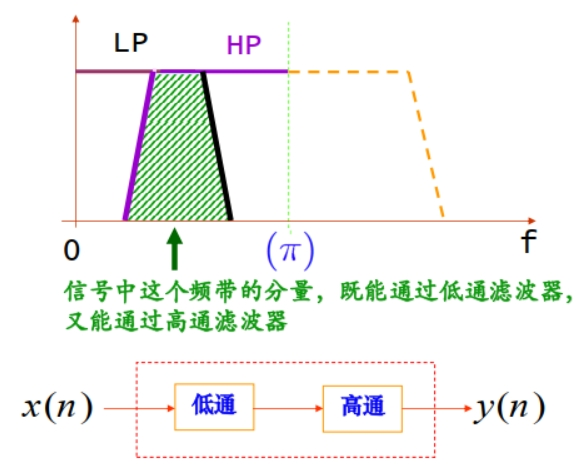
\includegraphics[width=0.6\textwidth]{chap4/img/band_pass_filter_cascade.png}
        \caption{带通滤波器级联}
        \label{fig:band-pass-filter-cascade}
    \end{figure}
    因此,
    \begin{align*}
        H_{\text{BP}}(\omega) & = H_{\text{LP}}(\omega) \cdot H_{\text{HP}}(\omega), \\
        h_{\text{BP}}(n) & = h_{\text{LP}}(n) * h_{\text{HP}}(n).
    \end{align*}
\end{note}

\subsubsection{高通 FIR 滤波器的设计}

高通 FIR 滤波器的设计与低通 FIR 滤波器的设计类似,只是将带通滤波器的中心频率移动到高频区域,
此时 $\omega_0 = \pi$。

\begin{exercise}
    根据下列指标设计高通 FIR 滤波器,写出其单位冲激响应函数 $h(n)$。
    \begin{figure}[H]
        \centering
        \begin{tabular}{|c|c|}
            \hline
            通带边缘频率:$8\;\mathrm{kHz}$ & 阻带边缘频率:$6\;\mathrm{kHz}$ \\
            \hline
            采样频率:$22\;\mathrm{kHz}$ & 阻带衰减:$40\;\mathrm{dB}$ \\
            \hline
        \end{tabular}
    \end{figure}
    供设计 FIR 滤波器时参考的各种窗函数性能如下图所示(若多种同时满足,则选序号最小的):
    \begin{figure}[H]
        \centering
        \begin{tabular}{|c|c|>{\centering\arraybackslash}p{5cm}|>{\centering\arraybackslash}p{4cm}|c|c|}
            \hline
            \textbf{序号} & \textbf{窗类型} & \makecell{\textbf{窗函数} \\ $(\abs{n} \le (N - 1) / 2)$} & \makecell{\textbf{窗内项数}\\(\text{T.W.} 是过渡带宽度)} & \textbf{阻带衰减} & \textbf{通带边缘增益} \\
            \hline
            1 & 矩形 & $1$ & $0.91 f_s / \text{T.W.}$ & $21$ & $-0.9$ \\
            \hline
            2 & 汉宁 & $0.5 + 0.5\cos(2\pi n / (N-1))$ & $3.32 f_s / \text{T.W.}$ & $44$ & $-0.06$ \\
            \hline
            3 & 哈明 & $0.54 + 0.46\cos(2\pi n / (N-1))$ & $3.44 f_s / \text{T.W.}$ & $55$ & $-0.02$ \\
            \hline
            4 & 布莱克曼 & $0.42 + 0.5\cos(2\pi n / (N-1)) + 0.08\cos(4\pi n / (N-1))$ & $5.98 f_s / \text{T.W.}$ & $75$ & $-0.0014$ \\
            \hline
        \end{tabular}
    \end{figure}
\end{exercise}

\begin{solution}
    首先考虑其对应的低通 FIR 滤波器,截止频率
    \begin{align*}
        f_c = \frac{22}{2} - 8 + \frac{1}{2} \times (8 - 6) = 4\;\mathrm{kHz},
    \end{align*}
    则
    \begin{align*}
        \omega_c = 2\pi \times \frac{f_c}{f_s} = 2\pi \times \frac{4}{22} = \frac{4\pi}{11}.
    \end{align*}
    计算得
    \begin{align*}
        h(n) = \frac{\sin(\omega_c n)}{\pi n} = \frac{\sin(4\pi n / 11)}{\pi n}.
    \end{align*}
    由阻带衰减为 $40\;\mathrm{dB}$ 知,应当选择汉宁窗。由于
    \begin{align*}
        N \ge 3.32 \times \frac{f_s}{\text{T.W.}} = 3.32 \times \frac{22}{8 - 6} = 36.52,
    \end{align*}
    故取 $N = 37$。则
    \begin{align*}
        w(n) = 0.5 + 0.5\cos\frac{2\pi n}{N - 1} = 0.5 + 0.5\cos\frac{\pi n}{18}.
    \end{align*}
    因此,高通 FIR 滤波器的冲激响应函数为
    \begin{align*}
        h'(n) = h(n) w(n) \cos(\pi n) = \frac{\sin(4\pi n / 11)}{\pi n} \left(0.5 + 0.5\cos\frac{\pi n}{18}\right) \cos(\pi n) \quad (\abs{n} \le 18).
    \end{align*}
    将其右移 $(N - 1) / 2 = 18$ 个单位,即得
    \begin{align*}
        h''(n) = \frac{\sin(4\pi (n - 18) / 11)}{\pi (n - 18)} \left(0.5 + 0.5\cos\frac{\pi (n - 18)}{18}\right) \cos(\pi (n - 18)) \quad (0 \le n \le 36).
    \end{align*}
\end{solution}

\begin{exercise}
    在以 $22\;\mathrm{kHz}$ 采集某种信号数据的过程中,虽然满足采样定理,但因受到环境的影响,
    采集的数据中夹杂了许多低频干扰信号。请选择一种满足条件的窗函数(若多种同时满足,
    则选序号较小的),设计一个高通 FIR 滤波器去除这些干扰信号。
    要求设计的高通滤波器的通带边缘频率为 $8\;\mathrm{kHz}$,
    过渡带宽度为 $2\;\mathrm{kHz}$,且至少满足阻带衰减 $45\;\mathrm{dB}$。
    请写出一种符合设计要求的滤波器的单位冲激响应函数 $h(n)$。
    \begin{figure}[H]
        \centering
        \begin{tabular}{|c|c|>{\centering\arraybackslash}p{5cm}|>{\centering\arraybackslash}p{4cm}|c|c|}
            \hline
            \textbf{序号} & \textbf{窗类型} & \makecell{\textbf{窗函数} \\ $(\abs{n} \le (N - 1) / 2)$} & \makecell{\textbf{窗内项数}\\(\text{T.W.} 是过渡带宽度)} & \textbf{阻带衰减} & \textbf{通带边缘增益} \\
            \hline
            1 & 矩形 & $1$ & $0.91 f_s / \text{T.W.}$ & $21$ & $-0.9$ \\
            \hline
            2 & 汉宁 & $0.5 + 0.5\cos(2\pi n / (N-1))$ & $3.32 f_s / \text{T.W.}$ & $44$ & $-0.06$ \\
            \hline
            3 & 哈明 & $0.54 + 0.46\cos(2\pi n / (N-1))$ & $3.44 f_s / \text{T.W.}$ & $55$ & $-0.02$ \\
            \hline
            4 & 布莱克曼 & $0.42 + 0.5\cos(2\pi n / (N-1)) + 0.08\cos(4\pi n / (N-1))$ & $5.98 f_s / \text{T.W.}$ & $75$ & $-0.0014$ \\
            \hline
        \end{tabular}
    \end{figure}
\end{exercise}

\begin{solution}
    首先考虑其对应的低通 FIR 滤波器,截止频率
    \begin{align*}
        f_c = \frac{22}{2} - 8 + \frac{1}{2} \times 2 = 4\;\mathrm{kHz},
    \end{align*}
    则
    \begin{align*}
        \omega_c = 2\pi \times \frac{f_c}{f_s} = 2\pi \times \frac{4}{22} = \frac{4\pi}{11}.
    \end{align*}
    计算得
    \begin{align*}
        h(n) = \frac{\sin(\omega_c n)}{\pi n} = \frac{\sin(4\pi n / 11)}{\pi n}.
    \end{align*}
    由阻带衰减为 $45\;\mathrm{dB}$ 知,应当选择哈明窗。由于
    \begin{align*}
        N \ge 3.44 \times \frac{f_s}{\text{T.W.}} = 3.44 \times \frac{22}{2} = 37.84,
    \end{align*}
    故取 $N = 39$。则
    \begin{align*}
        w(n) = 0.54 + 0.46\cos\frac{2\pi n}{N - 1} = 0.54 + 0.46\cos\frac{\pi n}{19}.
    \end{align*}
    因此,高通 FIR 滤波器的冲激响应函数为
    \begin{align*}
        h'(n) = h(n) w(n) \cos(\pi n) = \frac{\sin(4\pi n / 11)}{\pi n} \left(0.54 + 0.46\cos\frac{\pi n}{19}\right) \cos(\pi n) \quad (\abs{n} \le 19).
    \end{align*}
    将其右移 $(N - 1) / 2 = 19$ 个单位,即得
    \begin{align*}
        h''(n) = \frac{\sin(4\pi (n - 19) / 11)}{\pi (n - 19)} \left(0.54 + 0.46\cos\frac{\pi (n - 19)}{19}\right) \cos(\pi (n - 19)) \quad (0 \le n \le 38).
    \end{align*}
\end{solution}

\begin{exercise}
    根据下列指标设计高通 FIR 滤波器,写出其单位冲激响应函数 $h(n)$。
    \begin{figure}[H]
        \centering
        \begin{tabular}{|c|c|}
            \hline
            通带边缘频率:$8.8\;\mathrm{kHz}$ & 过渡带宽度:$4.4\;\mathrm{kHz}$ \\
            \hline
            采样频率:$22\;\mathrm{kHz}$ & 阻带衰减:$35\;\mathrm{dB}$ \\
            \hline
        \end{tabular}
    \end{figure}
    供设计 FIR 滤波器时参考的各种窗函数性能如下图所示(若多种同时满足,则选序号最小的):
    \begin{figure}[H]
        \centering
        \begin{tabular}{|c|c|>{\centering\arraybackslash}p{5cm}|>{\centering\arraybackslash}p{4cm}|c|c|}
            \hline
            \textbf{序号} & \textbf{窗类型} & \makecell{\textbf{窗函数} \\ $(\abs{n} \le (N - 1) / 2)$} & \makecell{\textbf{窗内项数}\\(\text{T.W.} 是过渡带宽度)} & \textbf{阻带衰减} & \textbf{通带边缘增益} \\
            \hline
            1 & 矩形 & $1$ & $0.91 f_s / \text{T.W.}$ & $21$ & $-0.9$ \\
            \hline
            2 & 汉宁 & $0.5 + 0.5\cos(2\pi n / (N-1))$ & $3.32 f_s / \text{T.W.}$ & $44$ & $-0.06$ \\
            \hline
            3 & 哈明 & $0.54 + 0.46\cos(2\pi n / (N-1))$ & $3.44 f_s / \text{T.W.}$ & $55$ & $-0.02$ \\
            \hline
            4 & 布莱克曼 & $0.42 + 0.5\cos(2\pi n / (N-1)) + 0.08\cos(4\pi n / (N-1))$ & $5.98 f_s / \text{T.W.}$ & $75$ & $-0.0014$ \\
            \hline
        \end{tabular}
    \end{figure}
\end{exercise}

\begin{solution}
    首先考虑其对应的低通 FIR 滤波器,截止频率
    \begin{align*}
        f_c = \frac{22}{2} - 8.8 + \frac{1}{2} \times 4.4 = 4.4\;\mathrm{kHz},
    \end{align*}
    则
    \begin{align*}
        \omega_c = 2\pi \times \frac{f_c}{f_s} = 2\pi \times \frac{4.4}{22} = \frac{2\pi}{5}.
    \end{align*}
    计算得
    \begin{align*}
        h(n) = \frac{\sin(\omega_c n)}{\pi n} = \frac{\sin(2\pi n / 5)}{\pi n}.
    \end{align*}
    由阻带衰减为 $35\;\mathrm{dB}$ 知,应当选择汉宁窗。由于
    \begin{align*}
        N \ge 3.32 \times \frac{f_s}{\text{T.W.}} = 3.32 \times \frac{22}{4.4} = 16.6,
    \end{align*}
    故取 $N = 17$。则
    \begin{align*}
        w(n) = 0.5 + 0.5\cos\frac{2\pi n}{N - 1} = 0.5 + 0.5\cos\frac{\pi n}{8}.
    \end{align*}
    因此,高通 FIR 滤波器的冲激响应函数为
    \begin{align*}
        h'(n) = h(n) w(n) \cos(\pi n) = \frac{\sin(2\pi n / 5)}{\pi n} \left(0.5 + 0.5\cos\frac{\pi n}{8}\right) \cos(\pi n) \quad (\abs{n} \le 8).
    \end{align*}
    将其右移 $(N - 1) / 2 = 8$ 个单位,即得
    \begin{align*}
        h''(n) = \frac{\sin(2\pi (n - 8) / 5)}{\pi (n - 8)} \left(0.5 + 0.5\cos\frac{\pi (n - 8)}{8}\right) \cos(\pi (n - 8)) \quad (0 \le n \le 16).
    \end{align*}
\end{solution}

\subsubsection{带阻 FIR 滤波器的设计}

带阻滤波器可以通过一个低通滤波器和一个高通滤波器并联实现。如图 \ref{fig:band-stop-filter-parallel} 所示。
\begin{figure}[H]
    \centering
    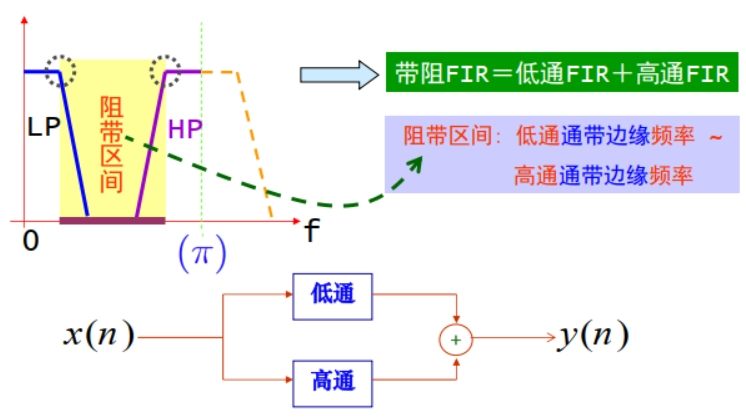
\includegraphics[width=0.6\textwidth]{chap4/img/band_stop_filter_parallel.png}
    \caption{带阻滤波器并联}
    \label{fig:band-stop-filter-parallel}
\end{figure}
因此,
\begin{align*}
    H_{\text{BS}}(\omega) & = H_{\text{LP}}(\omega) + H_{\text{HP}}(\omega), \\
    h_{\text{BS}}(n) & = h_{\text{LP}}(n) + h_{\text{HP}}(n).
\end{align*}
